% Banking 1B team progress deck (November 2026). Prepared by Kyaw Thi (Eric) Ha for the team.
\documentclass[aspectratio=169,10pt]{beamer}
% Banking 1B slide theme (by Kyaw Thi (Eric) Ha) — custom palette (no blue), IBM Plex type
\usepackage[sfdefault]{plex-sans}
\usepackage{plex-mono}
\usepackage{booktabs,tabularx,array,colortbl,graphicx,tikz,xcolor}
\usetikzlibrary{positioning,arrows.meta,calc}

\definecolor{ink}{HTML}{17211C}       % dark charcoal-green
\definecolor{paper}{HTML}{FBFBF8}     % light background
\definecolor{panel}{HTML}{ECEEE7}     % second background tone
\definecolor{body}{HTML}{3D4741}      % softened body text
\definecolor{muted}{HTML}{5E6862}
\definecolor{rule}{HTML}{D6DAD2}
\definecolor{emerald}{HTML}{16855A}   % accent 1
\definecolor{amber}{HTML}{A97A06}     % accent 2
\definecolor{mint}{HTML}{BFD9C8}      % light text on dark

\setbeamercolor{background canvas}{bg=paper}
\setbeamercolor{normal text}{fg=body,bg=paper}
\setbeamercolor{frametitle}{fg=ink,bg=paper}
\setbeamercolor{title}{fg=paper}
\setbeamercolor{structure}{fg=emerald}
\setbeamercolor{alerted text}{fg=emerald}
\setbeamercolor{itemize item}{fg=emerald}
\setbeamercolor{itemize subitem}{fg=amber}
\setbeamercolor{enumerate item}{fg=emerald}
\setbeamertemplate{navigation symbols}{}
\setbeamertemplate{itemize item}{\raisebox{0.18em}{\rule{0.42em}{0.42em}}}
\setbeamertemplate{itemize subitem}{\raisebox{0.22em}{\rule{0.3em}{0.3em}}}
\setbeamerfont{frametitle}{size=\LARGE,series=\bfseries}
\setbeamerfont{normal text}{size=\normalsize}
\setlength{\leftmargini}{1.1em}
\hyphenpenalty=10000 \exhyphenpenalty=10000
\newcolumntype{L}{>{\raggedright\arraybackslash}X}
\newcolumntype{B}[1]{>{\raggedright\arraybackslash\bfseries}p{#1}}

% Eyebrow (section label) above every frame title + page footer
\newcommand{\eyebrow}{}
\setbeamertemplate{frametitle}{%
  \vspace*{0.55cm}%
  {\usebeamercolor[fg]{structure}\scriptsize\bfseries\MakeUppercase{\eyebrow}\par}\vspace{0.12cm}%
  {\usebeamerfont{frametitle}\usebeamercolor[fg]{frametitle}\insertframetitle\par}%
  \vspace{0.05cm}}
\setbeamertemplate{footline}{%
  \hbox to \paperwidth{\hspace{0.9cm}{\color{muted}\tiny Banking 1B \textperiodcentered{} Fraud detection progress update \textperiodcentered{} November 2026}\hfill{\color{muted}\tiny\insertframenumber}\hspace{0.9cm}}\vspace{0.35cm}}
\setbeamersize{text margin left=0.9cm, text margin right=0.9cm}

\newcommand{\eb}[1]{\renewcommand{\eyebrow}{#1}}
\newcommand{\num}[1]{{\fontseries{b}\selectfont #1}}
\newcommand{\who}[1]{{\color{muted}\scriptsize #1}}

% A tinted card
\newcommand{\card}[3][panel]{%
  \begin{tikzpicture}\node[fill=#1,rounded corners=4pt,inner sep=9pt,text width=#2,align=left]{#3};\end{tikzpicture}}

% Big stat block: number, label
\newcommand{\stat}[3][emerald]{%
  \begin{minipage}[t]{0.3\linewidth}\raggedright{\color{#1}\fontsize{30}{32}\selectfont\bfseries #2}\\[2pt]{\small\color{body}#3}\end{minipage}}

\graphicspath{{figs/}}
\title{Online Payment Fraud Detection}

\begin{document}

% ---------------------------------------------------------------- 1 Title
{\setbeamercolor{background canvas}{bg=ink}\setbeamertemplate{footline}{}
\begin{frame}[plain]
\vspace*{0.5cm}
{\color{mint}\small\bfseries BREAK THROUGH TECH AI STUDIO \textperiodcentered{} BANKING 1B}\\[0.35cm]
{\color{paper}\fontsize{30}{34}\selectfont\bfseries Online Payment Fraud Detection\par}
\vspace{0.2cm}
{\color{mint}\Large Progress update: data, features, baselines and first neural networks\par}
\vspace{0.6cm}
{\color{paper}\small\bfseries Team}\\[2pt]
{\color{mint}\small Kyaw Thi (Eric) Ha \textperiodcentered{} Salamot Fakoya \textperiodcentered{} Jean Cho \textperiodcentered{} Jennifer Perez-Juarez \textperiodcentered{} Salvador Frias \textperiodcentered{} Susie Marrero \textperiodcentered{} Bianca Blevins}\\[0.35cm]
{\color{paper}\small\bfseries Challenge Advisor}\ {\color{mint}\small Debasmita Das}\qquad
{\color{paper}\small\bfseries AI Studio Coach}\ {\color{mint}\small Harshini Donepudi}\\[0.6cm]
{\color{mint}\scriptsize November 2026 \textperiodcentered{} IEEE-CIS Fraud Detection dataset \textperiodcentered{} all results on the validation period; holdout untouched}
\end{frame}}

% ---------------------------------------------------------------- 2 Where we are
\eb{Where we are}
\begin{frame}{Three stages done, evaluation under way}
\vspace{0.3cm}
\hspace*{0.7cm}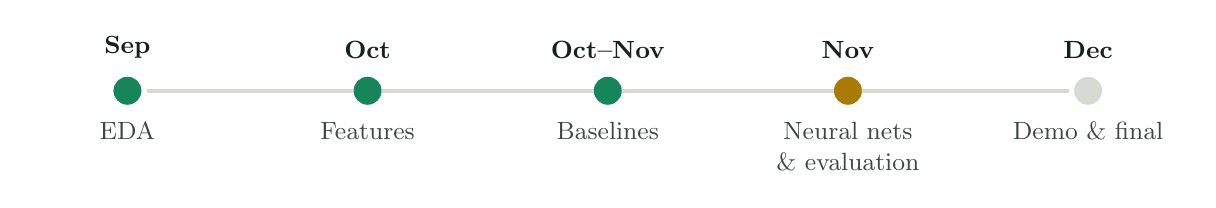
\begin{tikzpicture}[x=3.05cm]
  \foreach \i/\m/\t/\c in {0/Sep/EDA/emerald, 1/Oct/Features/emerald, 2/Oct--Nov/Baselines/emerald, 3/Nov/Neural nets \& evaluation/amber, 4/Dec/Demo \& final/rule}{
    \fill[\c] (\i,0) circle (5pt);
    \node[above=8pt, font=\small\bfseries, text=ink] at (\i,0) {\m};
    \node[below=8pt, font=\small, text=body, text width=2.3cm, align=center] at (\i,0) {\t};}
  \draw[rule, line width=1.5pt] (0.08,0) -- (3.92,0);
  \foreach \i/\c in {0/emerald,1/emerald,2/emerald,3/amber,4/rule} \fill[\c] (\i,0) circle (5pt);
\end{tikzpicture}

\vspace{0.7cm}
\begin{columns}[T]
\column{0.32\textwidth}\card[panel]{4.3cm}{{\color{ink}\bfseries Done}\\[3pt]\small Joined and explored the data, built two feature tables, trained logistic regression, LightGBM and XGBoost.}
\column{0.32\textwidth}\card[panel]{4.3cm}{{\color{ink}\bfseries This month}\\[3pt]\small Small neural networks, a same-machine comparison with LightGBM, blending and segment checks.}
\column{0.32\textwidth}\card[panel]{4.3cm}{{\color{ink}\bfseries Today we need}\\[3pt]\small Your view on the detection target and review capacity, and on what to tune before the holdout test.}
\end{columns}
\end{frame}

% ---------------------------------------------------------------- 3 Data and split
\eb{Data \& setup}
\begin{frame}{Fraud is rare, so we split by time and keep a final test untouched}
\vspace{0.2cm}
\stat{590,540}{labeled transactions (IEEE-CIS, 434 joined columns)}\hfill
\stat{3.5\%}{are fraud in the training period}\hfill
\stat[amber]{0.031}{average precision of random guessing on validation}

\vspace{0.45cm}

\begin{tikzpicture}
  \fill[emerald] (0,0) rectangle (10.4,0.62); \node[text=paper,font=\small\bfseries] at (5.2,0.31) {Train: 472,432 rows (first 80\%)};
  \fill[ink!70] (10.45,0) rectangle (11.75,0.62); \node[text=paper,font=\scriptsize\bfseries] at (11.1,0.31) {Val};
  \fill[amber] (11.8,0) rectangle (13.1,0.62); \node[text=ink,font=\scriptsize\bfseries] at (12.45,0.31) {Hold};
  \node[anchor=north west,font=\scriptsize,text=muted] at (0,-0.08) {earlier transactions $\rightarrow$ later transactions};
  \node[anchor=north east,font=\scriptsize,text=muted,align=right] at (13.1,-0.08) {59,054 validation \textperiodcentered{} 59,054 holdout};
\end{tikzpicture}

\vspace{0.25cm}
\small Every model learns only from older transactions and is judged on later ones, like real deployment. The holdout has \textbf{not been scored yet}: it is saved for the single final model.
\end{frame}

% ---------------------------------------------------------------- 4 EDA
\eb{Exploratory analysis \textperiodcentered{} whole team}
\begin{frame}{What the data told us}
\vspace{0.2cm}
\renewcommand{\arraystretch}{1.4}
\begin{tabularx}{\linewidth}{@{}B{4.3cm}L@{}}
\toprule
Fraud is rare & 3.51\% of training transactions. Accuracy would hide poor detection, so we use precision--recall metrics. \\
Product mix matters & Product C has an 11.3\% fraud rate; high-volume product W holds about 43\% of all fraud. \\
Missingness is a signal & 414 of 434 columns have gaps, in repeating blocks whose fraud rates differ. \\
Address gaps hide risk & Transactions with no billing address are 11.4\% of rows but 36.9\% of fraud, so we built a second account key for them. \\
\bottomrule
\end{tabularx}
\vspace{0.3cm}

\who{Source: combined EDA notebook and EDA summary notes.}
\end{frame}

% ---------------------------------------------------------------- 5 Features
\eb{Feature engineering \textperiodcentered{} Eric, Jean, Jennifer, Salamot, Salvador, Susie}
\begin{frame}{Two model-ready tables built only from past information}
\begin{columns}[T]
\column{0.55\textwidth}
\small
\begin{itemize}\setlength{\itemsep}{2pt}
\item \textbf{Frequency and out-of-time target encoding} for categories with many values
\item \textbf{Account history and velocity}: counts and amounts over 1\,h, 24\,h, 7 and 30 days, using strictly earlier transactions
\item \textbf{Missingness} flags per block and missingness-profile clusters
\item \textbf{Email, device and amount} features, \texttt{id\_14} timezone as a category
\item \textbf{Reduced V-column set} (drop near-duplicates, $|r| > 0.95$)
\end{itemize}
\column{0.42\textwidth}
\card[panel]{5.3cm}{{\color{ink}\bfseries Tree table}\ \ {\color{emerald}\bfseries 537 columns}\\[2pt]\small Categories and missing values kept as they are. Used by LightGBM and XGBoost.}\\[0.25cm]
\card[panel]{5.3cm}{{\color{ink}\bfseries Neural-net table}\ \ {\color{emerald}\bfseries 515 columns}\\[2pt]\small Log-scaled, clipped, filled, standardized; one-hot for small categories. Used by logistic regression and neural nets.}
\end{columns}
\end{frame}

% ---------------------------------------------------------------- 6 Metrics
\eb{How we evaluate}
\begin{frame}{One ranking score, plus the numbers a fraud team would feel}
\vspace{0.15cm}
\renewcommand{\arraystretch}{1.2}\small
\begin{tabularx}{\linewidth}{@{}B{4.0cm}Lp{2.0cm}@{}}
\toprule
Metric & Plain meaning & Better is \\
\midrule
Average precision (AP) & Main score. Summarizes precision across all catch rates; random $\approx$ 0.031 & higher \\
Recall at 1\% FPR & Share of fraud caught if we may flag only 1\% of legitimate customers & higher \\
TFPR at 50\% detection & Legitimate alerts per fraud caught when we catch half the fraud & lower \\
Top-5\% capture & Share of fraud found if analysts review only the riskiest 5\% & higher \\
\bottomrule
\end{tabularx}
\vspace{0.15cm}

\small All models use the team's shared \texttt{evaluate()} function on the same 59,054 validation transactions.
\end{frame}

% ---------------------------------------------------------------- 7 Baselines
\eb{Baseline models \textperiodcentered{} Jean, Bianca, Salamot, Salvador, Jennifer}
\begin{frame}{Boosted trees beat the linear baseline by a wide margin}
\vspace{0.1cm}
\renewcommand{\arraystretch}{1.25}\small
\begin{tabularx}{\linewidth}{@{}L rrrr@{}}
\toprule
\textbf{Model (validation, untuned)} & \textbf{AP} & \textbf{ROC-AUC} & \textbf{Recall @1\% FPR} & \textbf{Top-5\% capture}\\
\midrule
Logistic regression (numeric table) & 0.428 & 0.867 & 37.6\% & 50.8\% \\
XGBoost (integer-coded categories, 3 seeds) & 0.613 & -- & 53.1\% & -- \\
\rowcolor{panel} LightGBM (\texttt{all} features, tree table) & \textbf{0.632} & \textbf{0.931} & \textbf{56.4\%} & \textbf{68.4\%} \\
\bottomrule
\end{tabularx}
\vspace{0.35cm}
\begin{columns}[T]
\column{0.48\textwidth}\small
\textbf{\color{ink}Feature checks.} Removing engineered families (target encoding, behavior) changed AP in different directions across seeds: no consistent gain or loss yet, so nothing is dropped.
\column{0.48\textwidth}\small
\textbf{\color{ink}Leakage check.} Training on shuffled labels gives AP 0.033, the same as random (0.031). No sign of leakage in the label-free features.
\end{columns}
\vspace{0.15cm}
\who{Source: baseline modeling notebook, Sections 6d3, 8 and 13. XGBoost recall is seed 0.}
\end{frame}

% ---------------------------------------------------------------- 8 Statement
{\setbeamercolor{background canvas}{bg=emerald}\setbeamertemplate{footline}{}
\begin{frame}[plain]
\vspace*{1.6cm}
{\color{mint}\small\bfseries NOVEMBER \textperiodcentered{} SMALL NEURAL NETWORKS \textperiodcentered{} ERIC}\\[0.4cm]
{\color{paper}\fontsize{26}{31}\selectfont\bfseries Logistic regression adds up features in a straight line. Can a small neural network learn the combinations the trees find?\par}
\vspace{0.6cm}
{\color{paper}\normalsize Same 515-column table, same rows, same metrics. One change at a time.}
\end{frame}}

% ---------------------------------------------------------------- 9 What a small net is
\eb{Neural networks \textperiodcentered{} Eric}
\begin{frame}{What we trained}
\begin{columns}[T]
\column{0.5\textwidth}
\vspace{0.1cm}
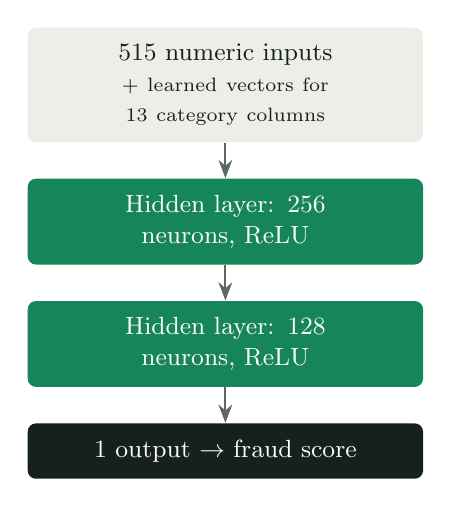
\begin{tikzpicture}[node distance=0.45cm, every node/.style={font=\small, rounded corners=3pt, inner sep=6pt, align=center}]
  \node[fill=panel,text=ink,text width=4.6cm] (in) {515 numeric inputs\\{\scriptsize + learned vectors for 13 category columns}};
  \node[fill=emerald,text=paper,text width=4.6cm,below=of in] (h1) {Hidden layer: 256 neurons, ReLU};
  \node[fill=emerald,text=paper,text width=4.6cm,below=of h1] (h2) {Hidden layer: 128 neurons, ReLU};
  \node[fill=ink,text=paper,text width=4.6cm,below=of h2] (out) {1 output $\rightarrow$ fraud score};
  \draw[-{Stealth},muted,thick] (in)--(h1); \draw[-{Stealth},muted,thick] (h1)--(h2); \draw[-{Stealth},muted,thick] (h2)--(out);
\end{tikzpicture}
\column{0.47\textwidth}\small
\textbf{\color{ink}Training.} Mini-batches of 2,048, Adam (lr 0.001), batch norm, dropout, early stopping on validation AP (patience 4).\\[0.25cm]
\textbf{\color{ink}Experiments.}
\begin{itemize}\setlength{\itemsep}{2pt}
\item 0 hidden layers (control)
\item Size: 64 \textperiodcentered{} 256--128 \textperiodcentered{} 512--256--128
\item Extra weight on fraud rows (5.2$\times$)
\item \textbf{Embeddings} for \texttt{card1}, \texttt{addr1}, email domains, device and browser
\end{itemize}
\vspace{0.1cm}
\who{About 1 minute per model on a laptop CPU.}
\end{columns}
\end{frame}

% ---------------------------------------------------------------- 10 Results bar
\eb{Neural networks \textperiodcentered{} results}
\begin{frame}{Hidden layers and embeddings each add real lift; trees still lead}
\centering
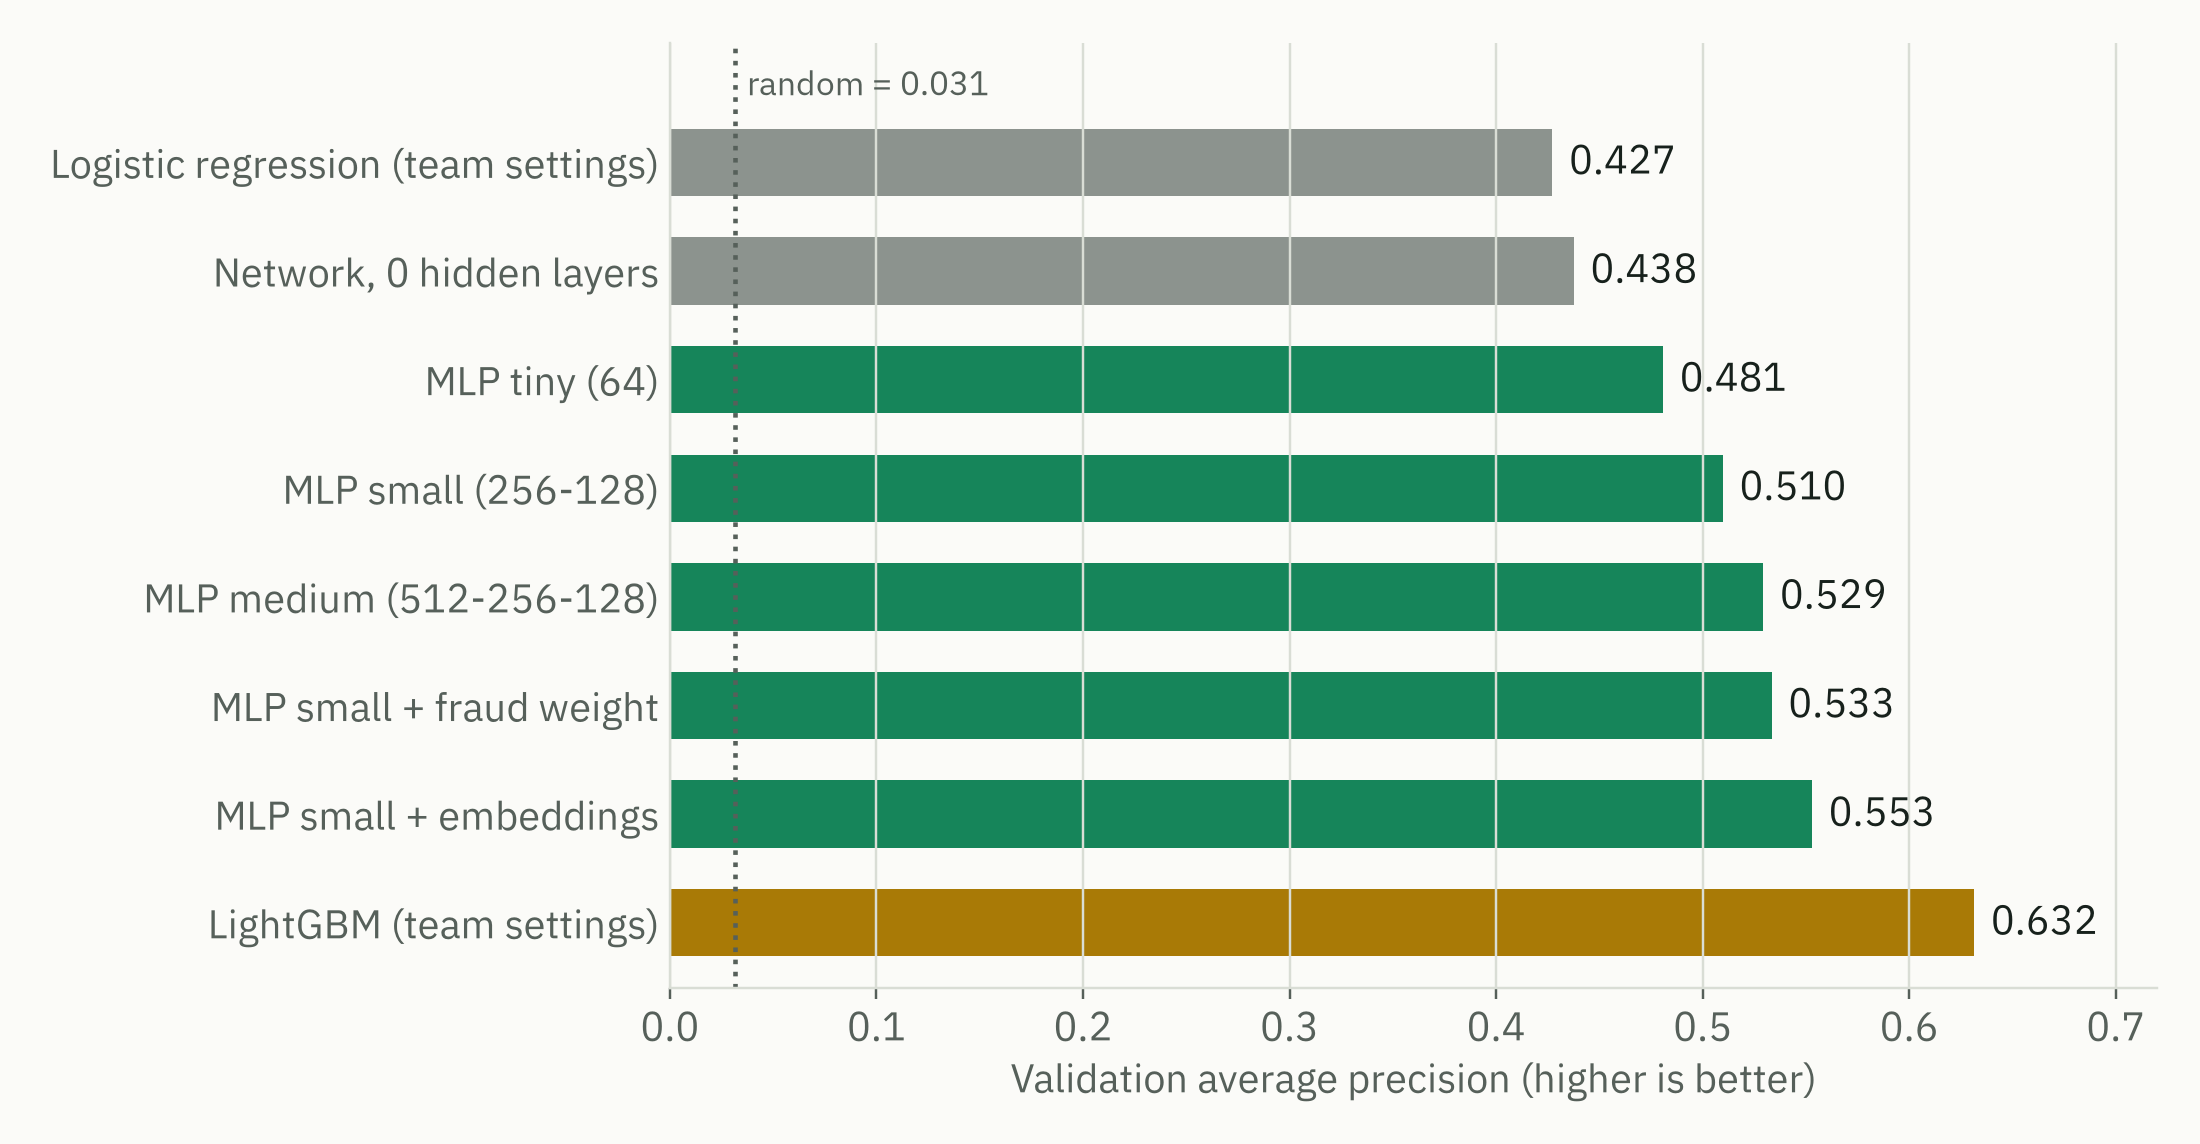
\includegraphics[width=0.66\linewidth]{fig_ap_bars.png}\\[-0.05cm]
\raggedright\who{Validation AP, seed 0, all models trained on the same machine and rows. Gray = linear, emerald = neural nets, amber = LightGBM (team settings).}
\end{frame}

% ---------------------------------------------------------------- 11 What we learned
\eb{Neural networks \textperiodcentered{} what helped}
\begin{frame}{What each change was worth}
\vspace{0.1cm}
\renewcommand{\arraystretch}{1.1}\small
\begin{tabularx}{\linewidth}{@{}B{4.6cm}rL@{}}
\toprule
Change & \textbf{AP} & What it means \\
\midrule
Training loop alone (0 hidden layers) & 0.438 & Matches logistic regression (0.427): the gains below come from hidden layers \\
Add one hidden layer (64) & 0.481 & Non-linear combinations help immediately \\
Bigger: 256--128 / 512--256--128 & 0.515 / 0.529 & Diminishing returns from size \\
Weight fraud rows 5.2$\times$ & 0.533 & +0.02 on one seed; promising, not yet confirmed \\
\rowcolor{panel} Embeddings for card, address, email, device & \textbf{0.560} & \textbf{+0.045}, the largest single gain (3-seed mean) \\
\bottomrule
\end{tabularx}
\vspace{0.15cm}

\small \textbf{\color{ink}Why embeddings help:} \texttt{card1} and \texttt{addr1} are ID codes; as plain numbers, ID 9500 looks ``bigger'' than 7919. An embedding gives each common ID its own learned vector.
\end{frame}

% ---------------------------------------------------------------- 12 Seeds
\eb{Neural networks \textperiodcentered{} is it real?}
\begin{frame}{The embedding gain is far larger than seed-to-seed noise}
\centering
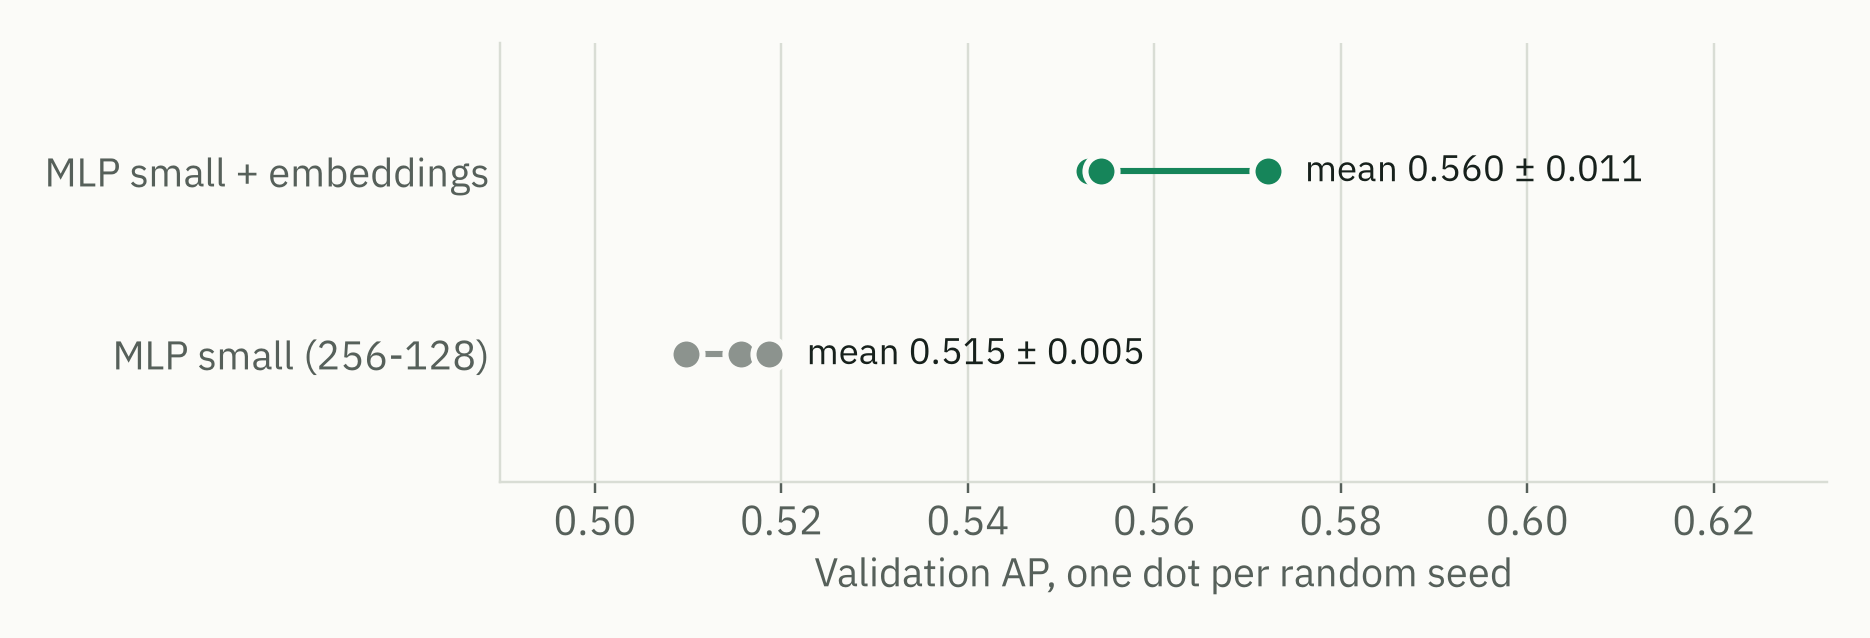
\includegraphics[width=0.78\linewidth]{fig_seeds.png}\\[0.1cm]
\raggedright\small Each dot is one training run with a different random start. The two ranges do not overlap: the worst embedding run (0.553) beats the best plain run (0.519).
\end{frame}

% ---------------------------------------------------------------- 13 Head to head
\eb{Comparison}
\begin{frame}{Best neural net against LightGBM, same validation rows}
\begin{columns}[T]
\column{0.5\textwidth}
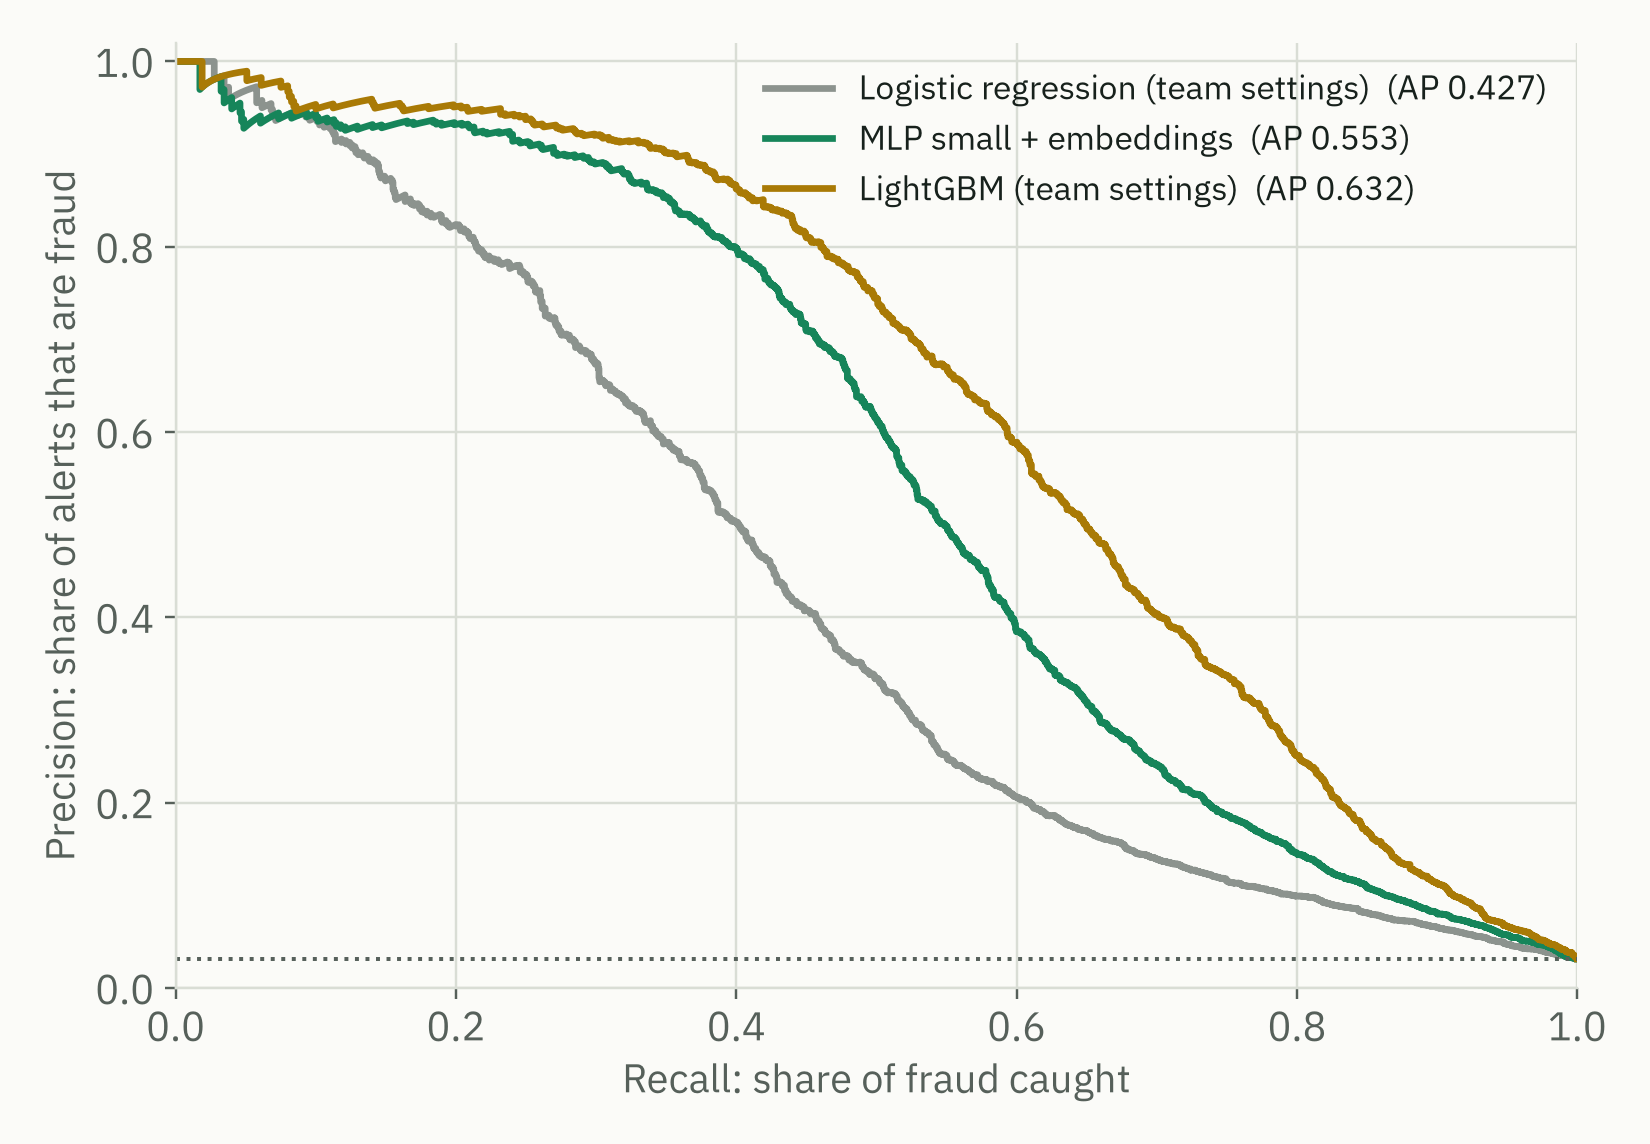
\includegraphics[width=\linewidth]{fig_pr_curves.png}
\column{0.48\textwidth}
\vspace{0.1cm}
\renewcommand{\arraystretch}{1.2}\small
\begin{tabularx}{\linewidth}{@{}L rrr@{}}
\toprule
& \textbf{LogReg} & \textbf{Net} & \textbf{LGBM}\\
\midrule
AP & 0.427 & 0.553 & \textbf{0.632} \\
ROC-AUC & 0.867 & 0.903 & \textbf{0.931} \\
Recall @1\% FPR & 37.6\% & 49.9\% & \textbf{56.4\%} \\
TFPR @50\% det. & 1.99 & 0.63 & \textbf{0.34} \\
TFPR @80\% det. & 9.08 & 5.88 & \textbf{2.98} \\
Top-5\% capture & 50.8\% & 60.6\% & \textbf{68.4\%} \\
\bottomrule
\end{tabularx}
\vspace{0.1cm}

\footnotesize The net closes about \textbf{60\%} of the gap from logistic regression to LightGBM. At 90\% detection: 14.3 / 11.3 / 7.8 legitimate alerts per fraud. \textbf{Only LightGBM stays under 10:1.}

\end{columns}
\end{frame}

% ---------------------------------------------------------------- 14 Blend
\eb{Comparison \textperiodcentered{} blending}
\begin{frame}{Does the network add anything on top of LightGBM?}
\begin{columns}[T]
\column{0.5\textwidth}
{\color{ink}\bfseries Rank-average blends}\\[4pt]
\renewcommand{\arraystretch}{1.2}\small
\begin{tabularx}{\linewidth}{@{}L rr@{}}
\toprule
\textbf{Net weight} & \textbf{AP} & \textbf{vs LightGBM}\\
\midrule
0\% (LightGBM alone) & 0.632 & -- \\
10\% & 0.628 & $-$0.004 \\
20\% & 0.623 & $-$0.008 \\
30\% & 0.619 & $-$0.013 \\
50\% & 0.608 & $-$0.023 \\
\bottomrule
\end{tabularx}\\[5pt]
\who{95\% time-block bootstrap intervals all stay below 0 (10\%: $-$0.007 to $-$0.0001).}
\column{0.46\textwidth}
{\color{ink}\bfseries Who catches which fraud (top 5\% reviewed)}\\[6pt]

\begin{tikzpicture}[x=0.185cm]
  \fill[ink!80] (0,0) rectangle (20.6,0.55);       % both 57.3
  \fill[amber] (20.65,0) rectangle (24.6,0.55);    % lgbm only 11.1
  \fill[emerald] (24.65,0) rectangle (25.8,0.55);  % net only 3.2
  \fill[rule] (25.85,0) rectangle (36,0.55);       % missed 28.4
\end{tikzpicture}\\[6pt]
\small
\textcolor{ink}{\rule{0.6em}{0.6em}} Both: 1,061 (57\%)\\
\textcolor{amber}{\rule{0.6em}{0.6em}} Only LightGBM: 205 (11\%)\\
\textcolor{emerald}{\rule{0.6em}{0.6em}} Only the net: 60 (3\%)\\
\textcolor{rule}{\rule{0.6em}{0.6em}} Missed by both: 525 (28\%)\\[6pt]
The net mostly finds frauds LightGBM already finds, so \textbf{blending does not help}. The 28\% both miss points to missing information, not model choice.
\end{columns}
\end{frame}

% ---------------------------------------------------------------- 15 Segments & calibration
\eb{Comparison \textperiodcentered{} where it works}
\begin{frame}{Segments and calibration}
\begin{columns}[T]
\column{0.56\textwidth}
{\color{ink}\bfseries AP within each segment (compare across a row)}\\[4pt]
\renewcommand{\arraystretch}{1.12}\footnotesize
\begin{tabularx}{\linewidth}{@{}L rrrr@{}}
\toprule
\textbf{Segment} & \textbf{Fraud} & \textbf{LogReg} & \textbf{Net} & \textbf{LGBM}\\
\midrule
Product C & 11.8\% & 0.731 & 0.756 & 0.804\\
Product R & 4.7\% & 0.724 & 0.814 & 0.858\\
Product W & 1.9\% & 0.116 & 0.356 & 0.461\\
Identity present & 8.9\% & 0.684 & 0.734 & 0.787\\
Identity missing & 1.9\% & 0.118 & 0.358 & 0.462\\
Address missing & 12.1\% & 0.738 & 0.758 & 0.806\\
\bottomrule
\end{tabularx}\\[5pt]
\footnotesize The net trails LightGBM in every segment; the gap is largest ($\approx$0.10) on product W and no-identity transactions. On product W it triples logistic regression's AP.
\column{0.4\textwidth}
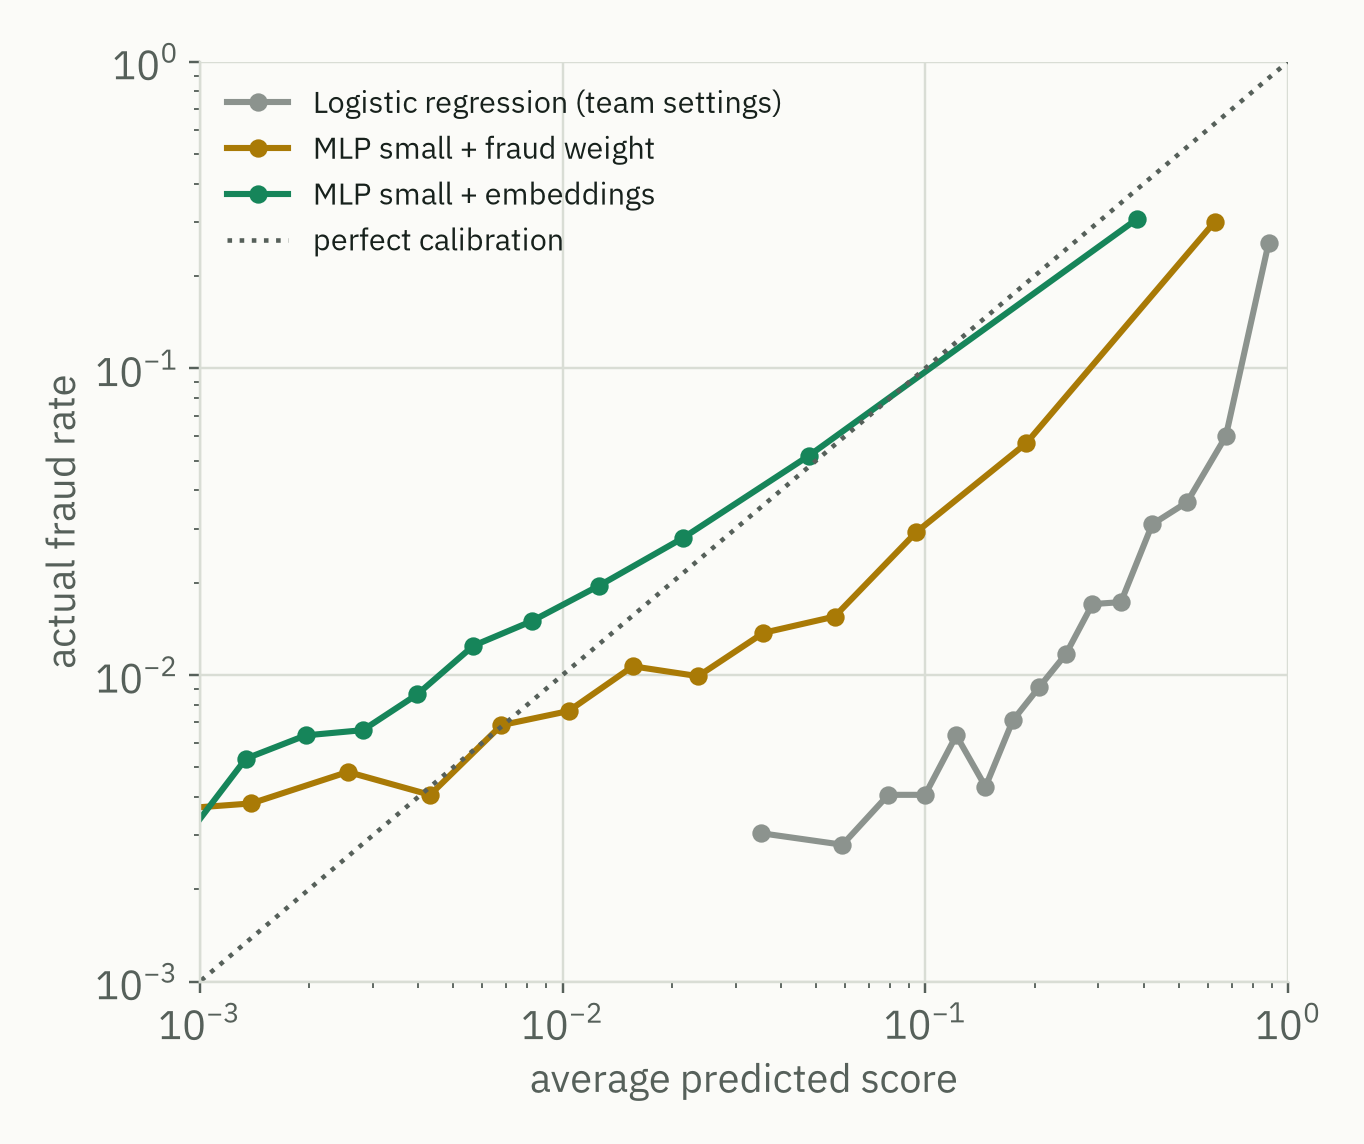
\includegraphics[width=0.92\linewidth]{fig_calibration.png}\\
\footnotesize Unweighted net: average score 0.033 vs 0.031 actual fraud rate, so its \textbf{scores read as real probabilities}. Weighting inflates them.
\end{columns}
\end{frame}

% ---------------------------------------------------------------- 16 Takeaways
\eb{Takeaways}
\begin{frame}{What we can say today}
\vspace{0.2cm}
\begin{columns}[T]
\column{0.32\textwidth}\card[panel]{4.3cm}{{\color{emerald}\fontsize{20}{22}\selectfont\bfseries +0.13 AP}\\[4pt]{\color{ink}\bfseries Small nets beat the linear baseline}\\[2pt]\small 0.427 $\rightarrow$ 0.560 on the same inputs, from hidden layers plus embeddings. Repeatable over 3 seeds.}
\column{0.32\textwidth}\card[panel]{4.3cm}{{\color{amber}\fontsize{20}{22}\selectfont\bfseries $-$0.07 AP}\\[4pt]{\color{ink}\bfseries LightGBM is still the strongest}\\[2pt]\small Ahead on every metric and segment; blending the net in makes it slightly worse.}
\column{0.32\textwidth}\card[panel]{4.3cm}{{\color{ink}\fontsize{20}{22}\selectfont\bfseries 28\%}\\[4pt]{\color{ink}\bfseries of fraud is missed by both}\\[2pt]\small At a 5\% review budget. The next gains are more likely from information than from a new algorithm.}
\end{columns}
\vspace{0.2cm}

\small\textbf{\color{ink}Recommendation:} keep LightGBM as the main model, keep the embedding network as the documented deep-learning baseline, and score the holdout once the model is frozen.\\[4pt]
\who{Caveats: validation is used for early stopping and model choice (slightly optimistic); most comparisons are one seed; no model is tuned yet.}
\end{frame}

% ---------------------------------------------------------------- 17 Next + questions
\eb{Next steps}
\begin{frame}{Plan to December, and questions for you}
\begin{columns}[T]
\column{0.52\textwidth}
{\color{ink}\bfseries Next steps}\\[4pt]\small
\begin{itemize}\setlength{\itemsep}{1pt}
\item Combine what helped (embeddings + fraud weighting), 3 seeds
\item Embeddings for the team's account keys
\item Study the 525 frauds both models miss, mostly product W
\item Tune LightGBM / XGBoost; confirm threshold with the TFPR table
\item Freeze model and features, then score the holdout once
\item December: demo, SHAP explanations, final README
\end{itemize}
\column{0.44\textwidth}
\card[panel]{5.5cm}{{\color{ink}\bfseries Questions for our advisor}\\[4pt]\small
1.\ Which detection target and review capacity should the final threshold use? (Validation stays under 10 legitimate alerts per fraud up to 90\% detection.)\\[4pt]
2.\ Is a small blend acceptable, or should the final model be a single model for explainability?\\[4pt]
3.\ Should we spend remaining time on tuning trees or on sequence models over account histories?}
\end{columns}
\end{frame}

\end{document}
